\documentclass[12pt]{article}

% Margins and spacing
\usepackage[margin=1in]{geometry}
\usepackage{setspace}
\onehalfspacing

% Packages
\usepackage{graphicx}
\usepackage{booktabs}
\usepackage{amsmath}
\usepackage{hyperref}
\usepackage{float}

\title{\textbf{BANA290 -- Assignment 2} \\
       \large AI Tool Impact on Worker Productivity: \\
       A Randomized Controlled Trial Analysis}
\author{Loan Operations Throughput Tracker \\
        March 2026 Audit Week}
\date{}

\begin{document}

\maketitle

% ============================================================
\section*{Interpretation of Results}
% ============================================================

\subsection*{Experimental Design and Randomization}

This analysis evaluates the causal impact of an AI PDF extraction
tool on loan processing clerk productivity and quality using data
from a Randomized Controlled Trial (RCT) conducted across two
sites -- Irvine Ops Center and Phoenix Processing Center -- during
the March 2026 audit week. A total of 141 clerk shift records were
included after cleaning, with 71 assigned to the treatment group
(AI tool) and 70 to the control group (manual processing).

The balance test confirmed that randomization was successful.
Pre-treatment characteristics -- years of experience, baseline
tasks per hour, baseline error rate, and training score -- showed
no statistically significant differences between groups (all
p-values $>$ 0.05), satisfying the \textbf{ignorability assumption}.
Table~\ref{tab:balance} reports the full balance test results.

\subsection*{SUTVA Justification}

The Stable Unit Treatment Value Assumption (SUTVA) requires that
no spillover effects exist between units and that only one version
of the treatment is applied. In this RCT, clerks process loan
applications independently on individual workstations. Each
clerk's output is self-contained -- one clerk's use of the AI
tool does not affect another's task queue or error rate. Clerks
were physically separated across Day and Evening shifts at two
geographically distinct sites, and assignments were randomized
within each site and queue. SUTVA is therefore satisfied.

\subsection*{Marginal Productivity Gain}

As shown in Figure~\ref{fig:boxplots}, clerks assigned to the AI
extraction tool completed an average of \textbf{79.23 tasks per
shift} compared to \textbf{70.56 tasks} for manual clerks -- a
statistically significant Average Treatment Effect (ATE) of
\textbf{+8.67 tasks per shift} ($p < 0.001$). This represents
approximately a \textbf{12.3\% productivity gain} directly
attributable to the AI tool, after baseline characteristics
are controlled for.

\subsection*{Quantity--Quality Trade-off}

The AI tool was also associated with a statistically significant
increase in error rates. Treatment clerks averaged an error rate
of \textbf{2.84\%} compared to \textbf{2.27\%} for control clerks,
yielding an ATE of \textbf{+0.57 percentage points} ($p = 0.0002$).
This suggests a modest \textbf{quantity--quality trade-off}: clerks
processed significantly more applications but with a small increase
in errors. The AI tool pre-fills fields from uploaded PDFs, which
may lead clerks to spend less time verifying individual entries,
introducing minor inaccuracies.

\subsection*{Implications for Firms}

The RCT design ensures that the estimated ATE is causal rather
than merely correlational. The productivity gains from broad AI
deployment are meaningful and statistically robust. However, firms
should not overlook the quality trade-off. A targeted intervention
combining AI assistance with a structured verification step --
prompting clerks to review pre-filled fields before submission
-- could preserve the speed advantage while closing the quality
gap. Firms should also monitor error rates continuously post-
deployment, particularly for junior clerks with lower experience
levels, as the trade-off may be more pronounced in that segment.

% ============================================================
\section*{Figures and Tables}
% ============================================================

\begin{figure}[H]
    \centering
    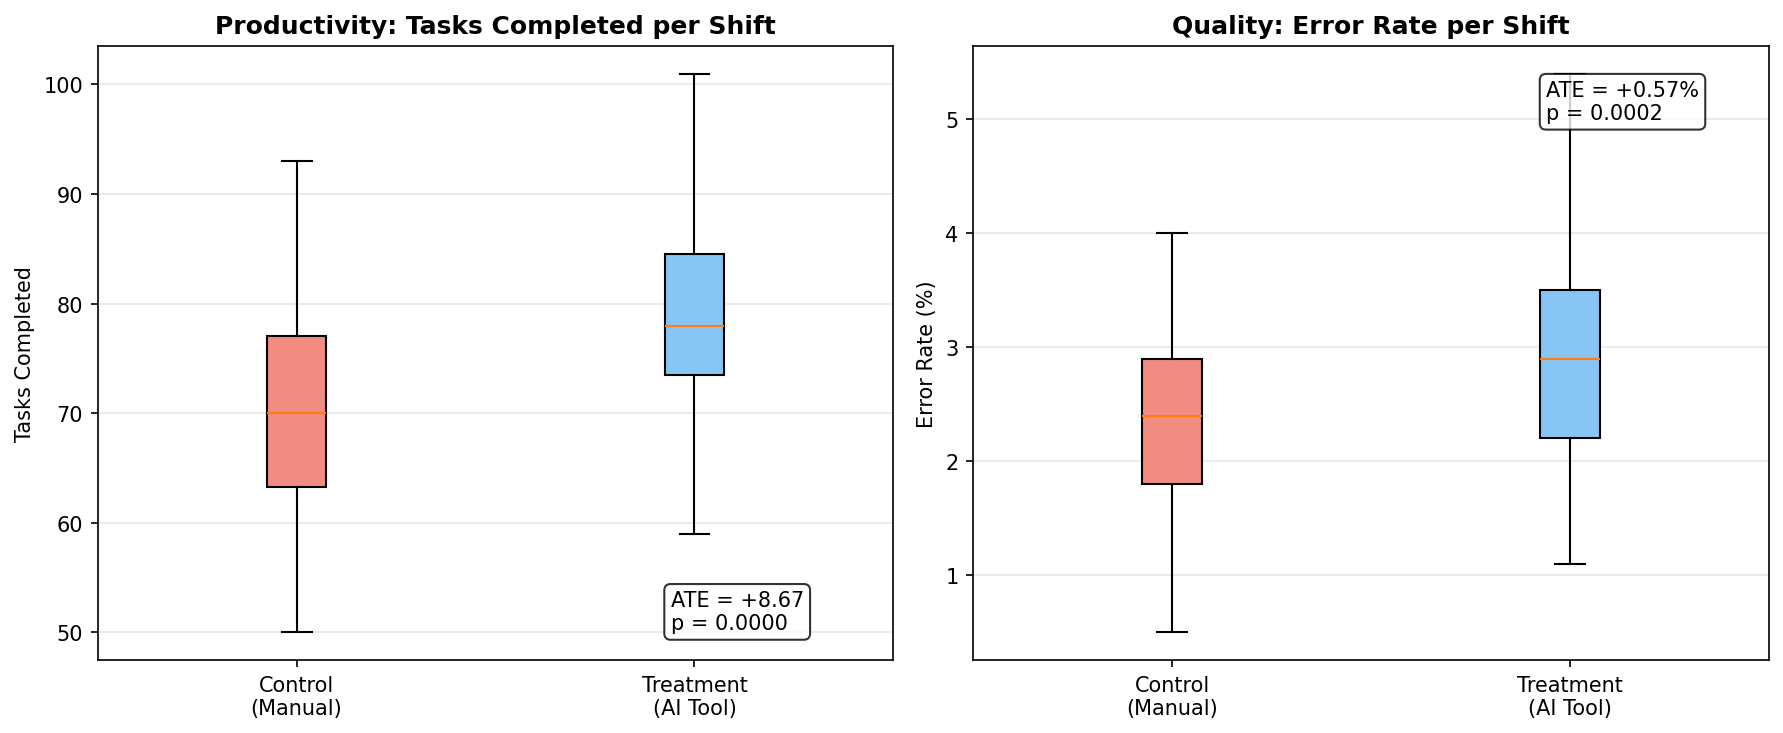
\includegraphics[width=\textwidth]{rct_boxplots.png}
    \caption{Left: Distribution of tasks completed per shift for
    treatment (AI Tool) and control (Manual) groups. Right:
    Distribution of error rates per shift. Both panels show the
    Average Treatment Effect (ATE) and p-value. The AI tool
    significantly increases productivity but also marginally
    increases error rates.}
    \label{fig:boxplots}
\end{figure}

\begin{table}[H]
    \centering
    \caption{Balance Test: Pre-Treatment Characteristics by Group}
    \begin{tabular}{lrrrrl}
        \toprule
        \textbf{Variable} & \textbf{Treatment} & \textbf{Control} &
        \textbf{t-stat} & \textbf{p-value} & \textbf{Balanced?} \\
        \midrule
        Years Experience  & 4.73 & 4.60 & 0.332 & 0.7401 & Yes \\
        Baseline Tasks/hr & 8.96 & 9.07 & -0.571 & 0.5691 & Yes \\
        Baseline Error \% & 2.19 & 2.19 & -0.017 & 0.9865 & Yes \\
        Training Score    & 87.1 & 87.5 & -0.289 & 0.7733 & Yes \\
        \bottomrule
    \end{tabular}
    \label{tab:balance}
\end{table}

\begin{table}[H]
    \centering
    \caption{Average Treatment Effect (ATE) Estimates}
    \begin{tabular}{lrrrr}
        \toprule
        \textbf{Outcome} & \textbf{Treatment Mean} &
        \textbf{Control Mean} & \textbf{ATE} & \textbf{p-value} \\
        \midrule
        Tasks Completed & 79.23 & 70.56 & $+$8.67 & $<$0.001 \\
        Error Rate (\%) & 2.84  & 2.27  & $+$0.57 & 0.0002   \\
        \bottomrule
    \end{tabular}
    \label{tab:ate}
\end{table}

\end{document}
